\section{Stokastisitet}
\subsection{Counting}
\begin{frame}
\begin{block}{Product Rule}
\begin{itemize}
\item Noe kan brytes ned i to aksjoner som kombineres med hverandre
\item For den ene finnes det $n_1$ muligheter, for den andre $n_2$
\item Det blir $n_1\cdot n_2$ kombinasjoner
\end{itemize}
\end{block}
\begin{block}{Eksempel}
\begin{itemize}
\item Det er to type maskiner som trenges
\item Den ene finnes 3 ganger, den andre 5 ganger
\item Hvor mange kombinasjoner maskintype 1, maskintype 2 finnes det?
\item $5\cdot 3=15$
\end{itemize}
\end{block}
\end{frame}

\begin{frame}
\begin{block}{Sum Rule}
\begin{itemize}
\item Noe kan gjøres på enten en av $n_1$ måter, eller en av $n_2$ måter
\item Det finnes ingen element som er både i $n_1$ og i $n_2$
\item Det blir $n_1+n_2$ muligheter å gjøre det
\end{itemize}
\end{block}
\begin{block}{Eksempel}
\begin{itemize}
\item En student skal velge masteroppgaven sin
\item Hun liker tre fagområder
\item I område $n_1$ finnes det 5 teamer, i $n_2$ 3 temaer, i område $n_3$ er det 8
\item Det er $5+3+8=16$ temaer å velge fra
\end{itemize}
\end{block}
\end{frame}

\begin{frame}
\begin{block}{Subtraction Rule}
\begin{itemize}
\item Ligner \textit{Sum rule}, men flere elementer er i flere grupper
\item Noe kan gjøres på enten en av $n_1$ måter, eller en av $n_2$ måter, men noen er i både $n_1$ og $n_2$
\item Det blir $n_1+n_2-felles(n_1,n_2)$ muligheter
\end{itemize}
\end{block}
\begin{block}{Eksempel}
\begin{itemize}
\item På fredag er det amerikansk-norsk folkefest
\item Det er 22 amerikanere og 18 nordmenn som meldte seg på
\item 3 av dem er både norsk og amerikansk
\item Det er $22+18-3=37$ personer som deltar
\end{itemize}
\end{block}
\end{frame}

\begin{frame}
\begin{block}{Division Rule}
\begin{itemize}
\item Det er $n$ måter å gjøre noe, men egentlig finnes det for hver måte minst $d$ lignende måter
\item Det blir da $n/d$ forskjellige muligheter
\end{itemize}
\end{block}
\begin{block}{Eksempel}
\begin{itemize}
\item I en fornøyelsespark for katter blir det talt 400 beiner. Mennesker og andre dyr har ikke lov å være i fornøyelsesparken
\item Hver katt har eksakt fire bein
\item Det betyr det er $400/4=100$ katter
\end{itemize}
\end{block}
\end{frame}

\subsection*{Kombinatorikk}
\begin{frame}{Permutasjon? Kombinasjon? Variasjon? Hæ?}
\begin{enumerate}
\item Blir alle elementer med?
	\begin{itemize}
	\item Ja: Permutasjon
	\item Nei: Variasjon eller Kombinasjon
	\end{itemize}
\item (Permutasjon, Kombinasjon) Er rekkefølgen viktig?
	\begin{itemize}
	\item Ja: Variasjon
	\item Nei: Kombinasjon
	\end{itemize}
\item Finnes det elementer flere ganger?
	\begin{itemize}
	\item Permutasjon uten repetisjon: $n!$
	\item Permutasjon med repetisjon: $\frac{n!}{r!\cdot s!\cdot t!}$
	\item Kombinasjon uten repetisjon: $\binom{n}{k}$
	\item Kombinasjon med repetisjon: $ \binom{(n+k-1)}{k}$
	\item Variasjon uten repetisjon: $\frac{n!}{(n-k)!}$
	\item Variasjon med repetisjon: $n^k$
	\end{itemize}
\end{enumerate}
\end{frame}

\begin{frame}{Eksempler}
\begin{block}{Eksempel 1}
\begin{itemize}
\item 7 personer må fotograferes. Hvor mange kombinasjoner finnes det å ordne dem på bildet?
\item Alle elementer blir med, ingen repetisjon 
\item Permutasjon uten repetisjon: $n!=7!=720$
\end{itemize}
\end{block}

\begin{block}{Eksempel 2}
\begin{itemize}
\item Hvor mange måter finnes det for å ordne bokstavene \textit{Mississippi}?
\item Alle elementer blir med, men repetisjon (permutasjon)
\item $\frac{n!}{r!\cdot s!\cdot t!} =  \frac{11!}{4!\cdot 4!\cdot 2!}=34650$
\end{itemize}
\end{block}
\end{frame}

\begin{frame}{Enda flere eksempler}
\begin{block}{Eksempel 3}
\begin{itemize}
\item Det er 7 personer og 3 tilfeldige av dem skal få en pris. Hvor mange kombinasjoner finnes det?
\item Ikke alle elementer blir med, ingen repetisjon, rekkefølgen ikke viktig 
\item Kombinasjon uten repetisjon: $\binom{n}{k}=\binom{7}{3}=\frac{7!}{3!\cdot 4!}=35$
\end{itemize}
\end{block}

\begin{block}{Eksempel 4}
\begin{itemize}
\item Vi har 5 typer is og skal spise 3 av dem. Vi er opptatt av rekkefølgen for best smak.
\item Ikke ealle lementer blir med, rekkefølge viktig, med repetisjon
\item $n^k=5^3=125$
\end{itemize}
\end{block}
\end{frame}

\subsection*{Spørretid}
\begin{frame}{Spørsmål?}
    \begin{figure}
        \centering
        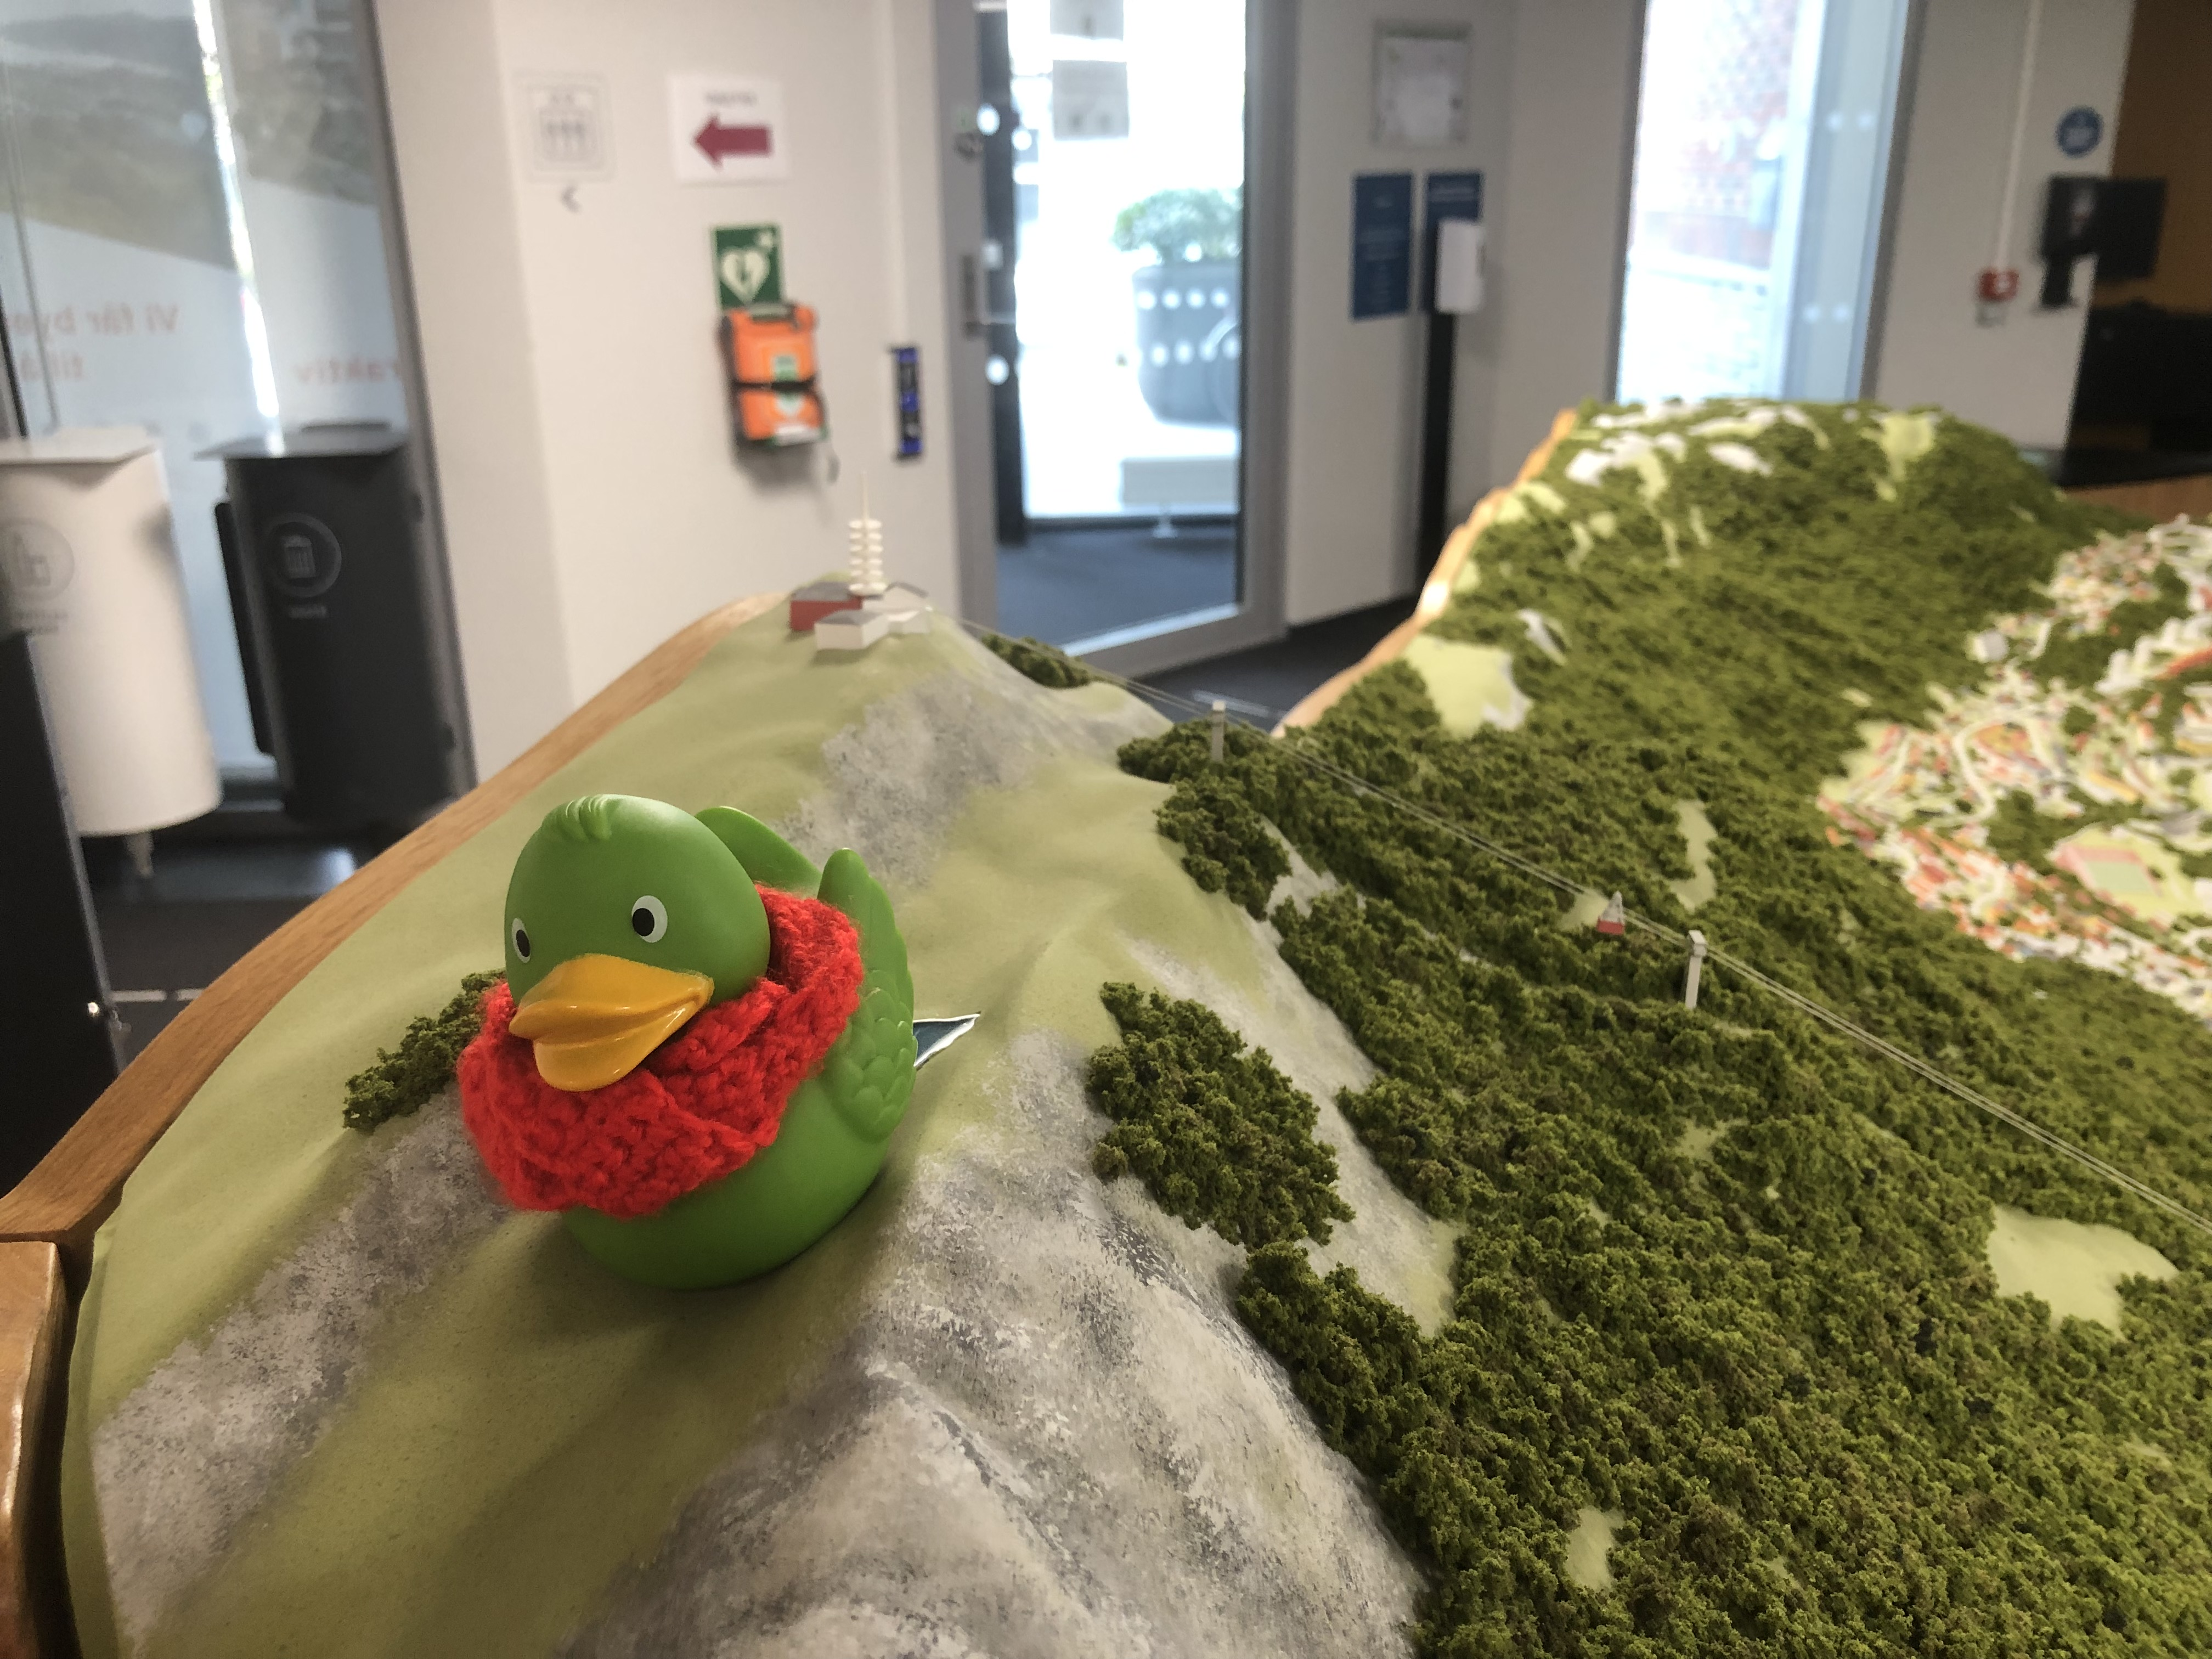
\includegraphics[height = 4.9cm]{images/guillaume11.jpg}
        \caption{Guillaume på Ulriken}
        \label{fig:guillaume11}
    \end{figure}
\end{frame}

\subsection{Sannsynligheter}
\begin{frame}{Definisjoner}
\begin{itemize}
\item \textbf{Utfallsrom: }Alle mengder som har en sannsynlighet
\item \textbf{S: }Alle mulige utfall
\item \textbf{E: }Alle ønskete utfall
\item $E \subseteq S$: alle ønskete utfall er en del av alle mulige utfall
\item \textbf{Sannsynlighet: }$P(E)=\frac{|E|}{|S|}$
\item $0 \leq P(E) \leq 1$
\item $P(S)=1$
\item $P(\overline{E})=1-P(E)$
\end{itemize}
\end{frame}

\begin{frame}{Regneregler}
\begin{itemize}
\item $P(A\cup B)=P(A)+P(B)-P(A\cap B)$ (tilsvarer subtraction rule)
\item $P(A\cap B)=P(A)\cdot P(B)$ hvis A,B statistisk uavhengig (tilsvarer multiplication rule)
\item $\sum_{s\in S} P(s) = 1 $ (summen av alle ting som kan skje har sannsynlighet 1)
\item \textbf{Betinget sannsynlighet: }$P(A|B)=\frac{P(A\cap B)}{P(B)}$ (Sannsynlighet av A etter at B skjedde)
\item \textbf{Bayes Rule: }$P(A|B)=\frac{P(B|A)\cdot P(A)}{P(B)}$
\end{itemize}
\end{frame}

\begin{frame}{Eksempler}
\begin{block}{Terninger}
\begin{itemize}
\item Det er to terninger, den ene er vanlig med 6 jevne sider
\item Den andre har tallene $\{3,4,5,5,6,6\}$
\item Hvor stor er sannsynligheten at vi kaster en 7 med begge terninger?
\item Det er $6\cdot 6$ mulige kombinasjoner
\item Det er fire måter å få det til:
\begin{itemize}
\item Terning 1: 1, Terning 2: 6 (finnes to ganger)
\item Terning 1: 2, Terning 2: 5 (finnes to ganger)
\item Terning 1: 3, Terning 2: 4
\item Terning 1: 4, Terning 2: 3
\end{itemize}
\item $P(sum=7)=\frac{6}{36}=\frac{1}{6}$
\end{itemize}
\end{block}
\end{frame}

\begin{frame}{Eksempler}
\begin{block}{Kortspill}
\begin{itemize}
\item Vi har et vanlig kortspill med 32 kort (4 farger, $\{7,8,9,10,J,Q,K,A\}$)
\item Hva er sannsynligheten at vi trekker et hjerte eller en konge?
\item Hva er sannsynligheten at en av disse kortene er 7,8 eller 9?
\item Det er 4 konger, 8 hjerter, en av dem er begge deler
\item $P(Konge\cup Hjerte)=\frac{8+4-1}{32}=\frac{11}{32}$
\item Blant disse er det 3 kort som er 7,8 eller 9
\item $P(7,8,9|Konge\cup Hjerte)=P((7,8,9)\cap(Konge\cup Hjerte))=\frac{3}{11}$
\end{itemize}
\end{block}
\end{frame}

\begin{frame}{\textit{Vierfeldertafel} (WANTED: norsk eller engelsk begrep)}
\begin{table}[h!]
\centering
\label{tab:prob_two_events}
\begin{tabular}{l|ll|l}
\cline{2-3}
                            & $A$            & $\overline{A}$            &                               \\ \hline
\multicolumn{1}{|l|}{$B$}   & $P(A\cap B)$   & $P(\overline{A}\cap B)$   & \multicolumn{1}{l|}{$P(B)$}   \\
\multicolumn{1}{|l|}{$\overline{B}$} & $P(A\cap \overline{B})$ & $P(\overline{A}\cap \overline{B})$ & \multicolumn{1}{l|}{$P(\overline{B})$} \\ \hline
                            & $P(A)$         & $P(\overline{A})$         & \multicolumn{1}{l|}{$1$}      \\ \cline{2-4} 
\end{tabular}
\caption{To hendelser A og B i en \textit{Vierfeldertafel}}
\end{table}
\begin{itemize}
\item Det er to spalter og to rekker, hver for en hendelse og motsetningen
\item I alle retninger kan man summe ting sammen
\item Det trenges bare tre utfylte felter for å regne ut resten
\end{itemize}
\end{frame}

\begin{frame}{\textit{Vierfeldertafel} (WANTED: norsk eller engelsk begrep)}
\begin{columns}
 \begin{column}{0.38\textwidth}
\begin{table}[h!]
\centering
\caption{Eksempel \textit{Vierfeldertafel}}
\label{tab:fourfold_eksempel1}
\begin{tabular}{l|ll|l}
\cline{2-3}
                            & $A$            & $A^C$            &                               \\ \hline
\multicolumn{1}{|l|}{$B$}   & 0.4   &     & \multicolumn{1}{l|}{0.533}   \\
\multicolumn{1}{|l|}{$B^C$} &   & 0.292 & \multicolumn{1}{l|}{} \\ \hline
                            &          &          & \multicolumn{1}{l|}{$1$}      \\ \cline{2-4} 
\end{tabular}
\end{table}

\begin{table}[h!]
\centering
%\caption{Eksempel \textit{Vierfeldertafel} ferdig utfylt}
\label{tab:fourfold_eksempel2}
\begin{tabular}{l|ll|l}
\cline{2-3}
                            & $A$            & $A^C$            &                               \\ \hline
\multicolumn{1}{|l|}{$B$}   & 0.4   & 0.133    & \multicolumn{1}{l|}{0.533}   \\
\multicolumn{1}{|l|}{$B^C$} & 0.175  & 0.292 & \multicolumn{1}{l|}{0.467} \\ \hline
                            & 0.575         & 0.425         & \multicolumn{1}{l|}{$1$}      \\ \cline{2-4} 
\end{tabular}
\end{table}
 \end{column}
 \begin{column}{0.58\textwidth}
\begin{itemize}
\item Det er gitt tre verdier, $P(B)$, $P(A\cap B)$, $P(A^C\cap B^C)$
\item Resten kan regnes ut ved summeformalen
\item Eksempel: $P(A^C\cap B)=P(A\cap B)-P(B)=0.533-0.4=0.133$
\item Kan brukes for å finne andre ting
\item Betinget sannsynlighet: $P(A|B)=\frac{P(A\cap B)}{P(B)}=\frac{0.4}{0.533}=0.75$
\end{itemize}
 \end{column}
\end{columns}
\end{frame}

\subsection*{Spørretid}
\begin{frame}{Spørsmål?}
    \begin{figure}
        \centering
        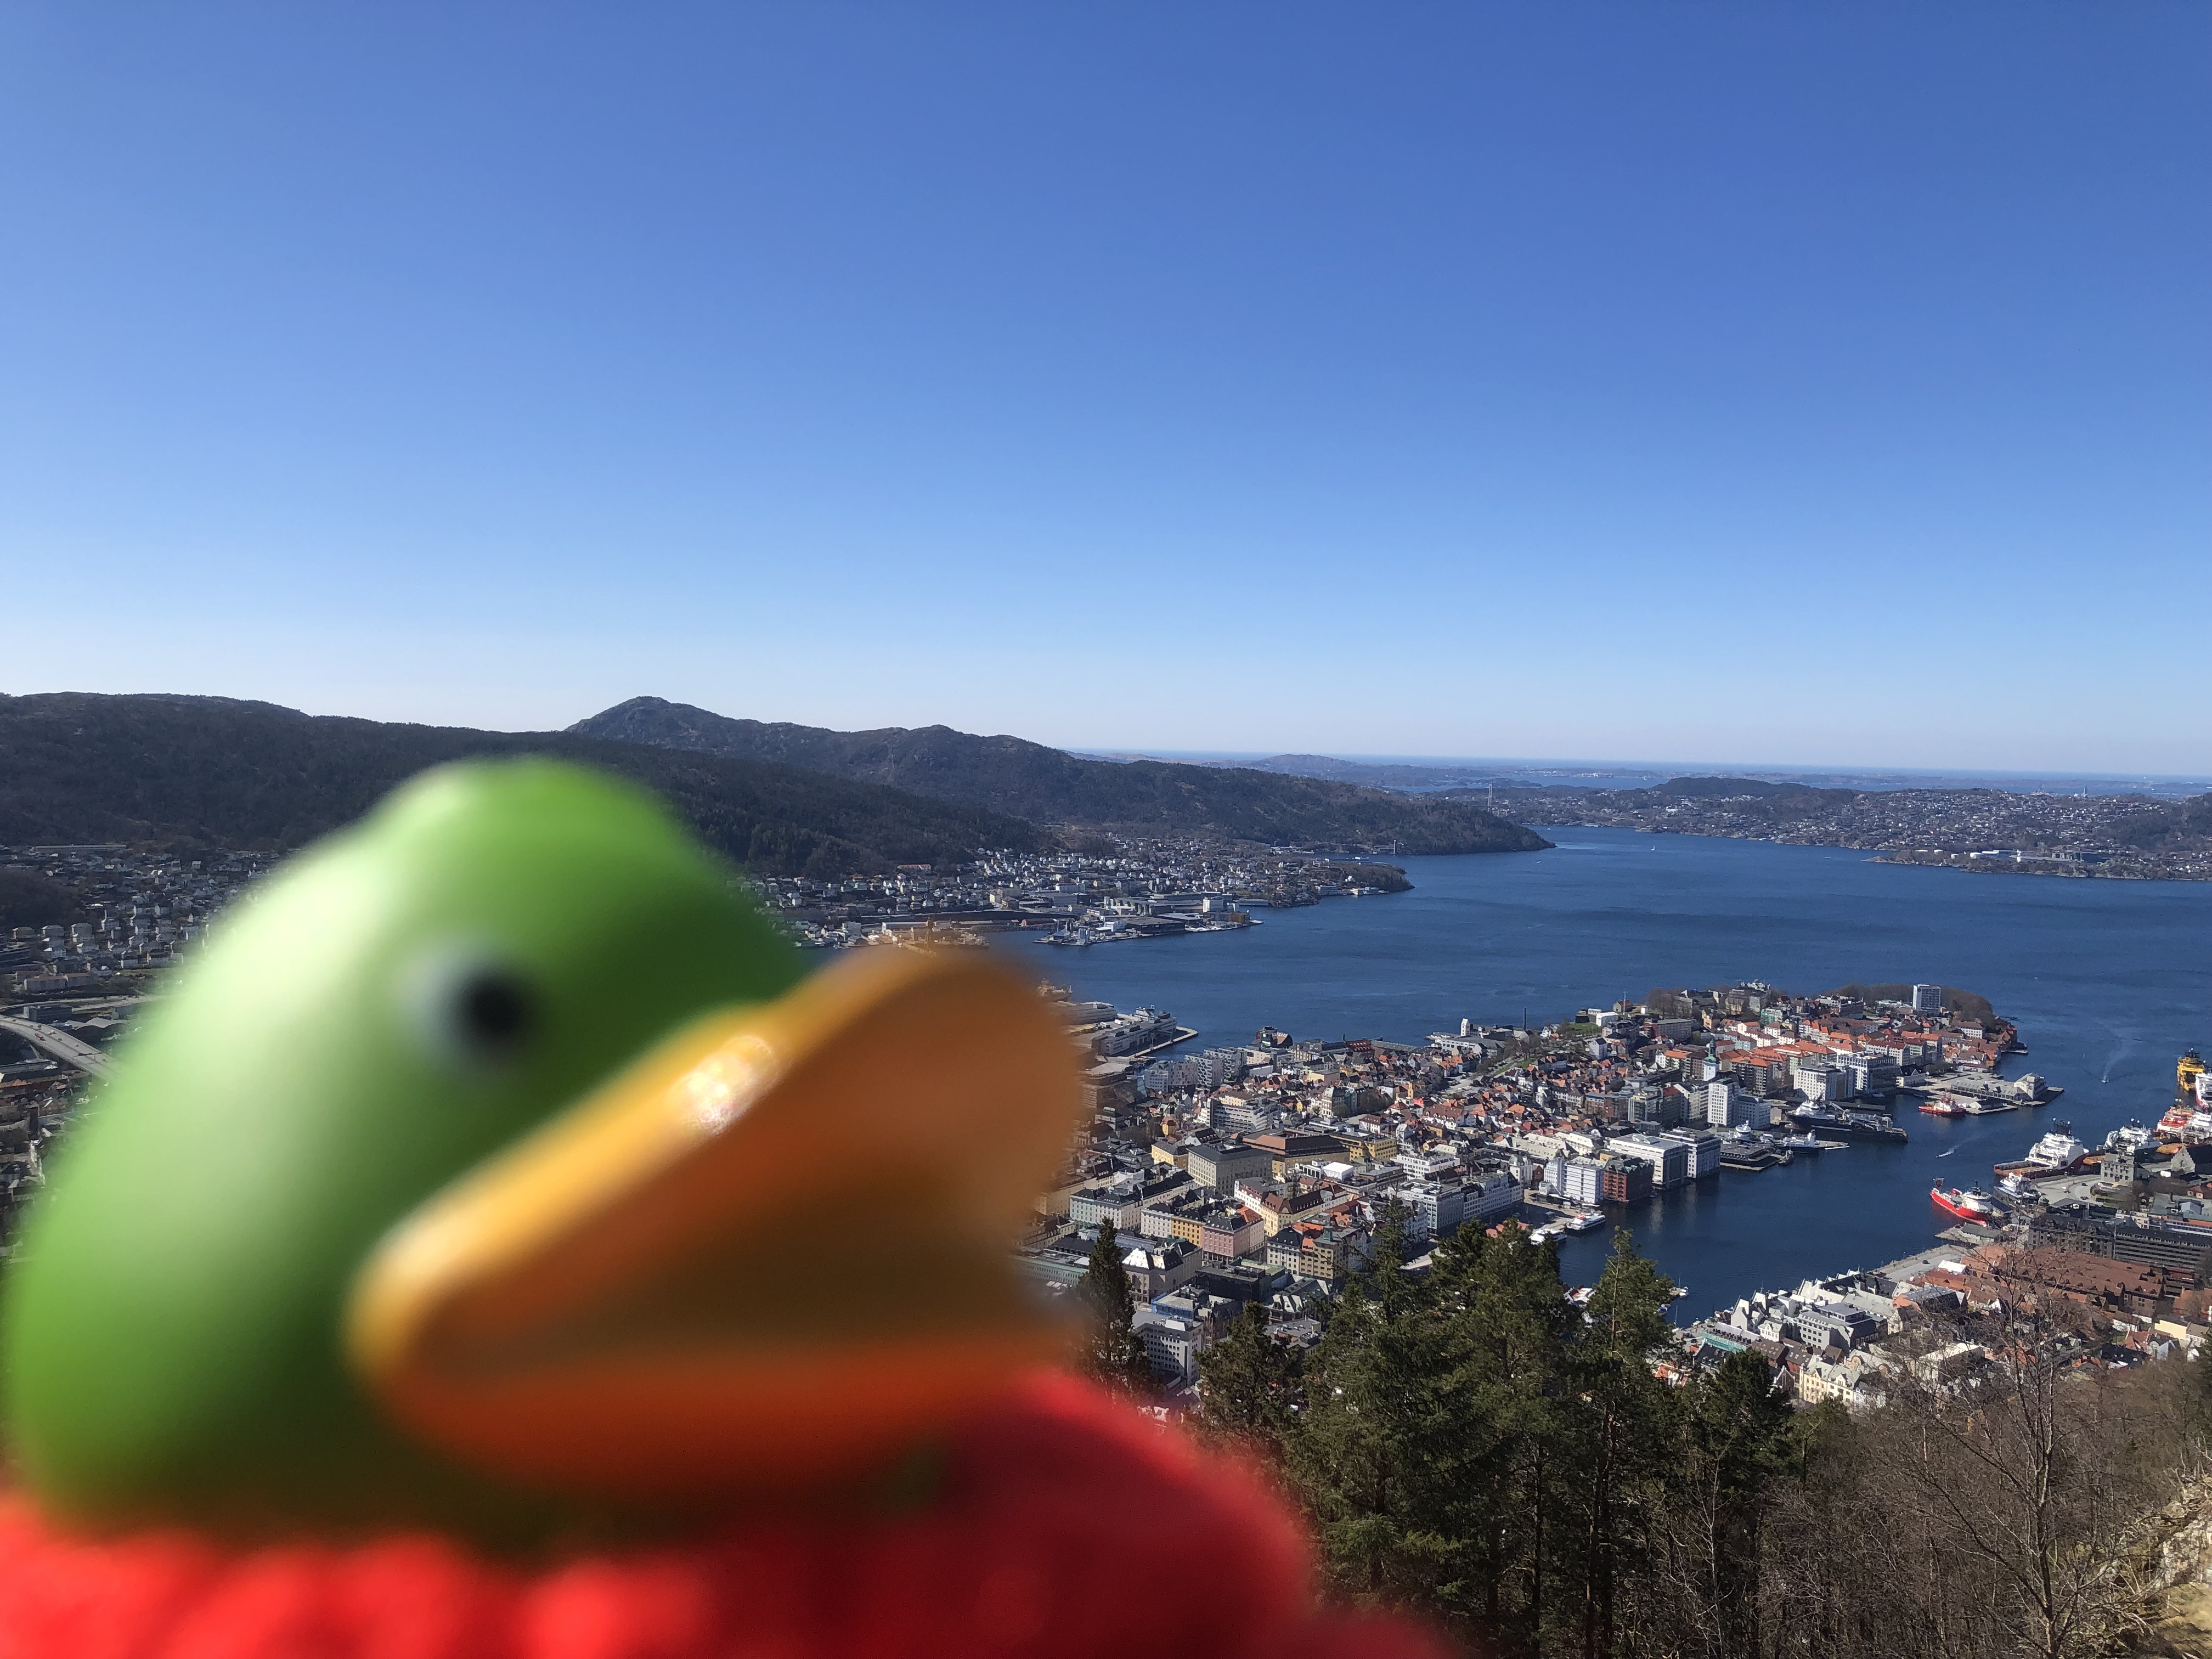
\includegraphics[height = 4.9cm]{images/guillaume10.jpg}
        \caption{Guillaume på Fløyen}
        \label{fig:guillaume10}
    \end{figure}
\end{frame}


